\chapter{Technologie i pojęcia wykorzystane w projekcie  }
\label{cha:Technologie}
W poniższym rozdziale przedstawiono zagadnienia 

\section{Obraz całkowy}
\label{sec:IntegralImage}
Obraz całkowy (z ang. \textit{Integral Image} \cite{ViolaJonesIntegralImage}) to struktura danych wykorzystywana w celu efektywnej i szybkiej generacji sum pikseli dla podanego regionu obrazu. Dowolny piksel \textit{(x, y)} obrazu \textit{I} może zostać przedstawiony jako suma wszystkich pikseli na lewo oraz powyżej \textit{(x, y)}:
\begin{equation}
\textit{Obraz całkowy}(x^{'},y^{'}) = \sum_{x<x^{'},y<y^{'}}^{}I(x,y).
\end{equation}

Użycie takiej reprezentacji umożliwia uzyskanie sumy pikseli dowolnego obszaru obrazu w stałym czasie, bez względu na jego rozmiar. Dodatkowo wyliczenie obrazu całkowego następuje w pojedynczym przejściu po pikselach. Wynika to z faktu, że kolejne elementy struktury są tworzone na podstawie już istniejących. Przykład wykorzystania obrazu całkowego  przedstawiono na rysunku \ref{im: Integral Image} 

\begin{figure}[h]
	%\centering
	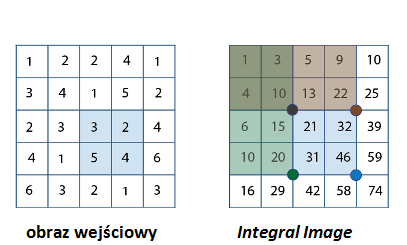
\includegraphics[width=12cm]{integral_image}
	\centering
	\caption{Zasada wyliczania obrazu całkowego}
	\label{im: Integral Image}
\end{figure}    

Wyliczenie sumy wyróżnionego regionu na obrazie wejściowym można zastąpić operacjami na obrazie całkowym. Sumę obszaru można uzyskać korzystając z czterech wartości powyżej oraz na lewo od zaznaczonych kropek: \textit{46 - 22 - 20 + 10 = 14}. Jak nietrudno obliczyć, wynik ten jest równy sumie zaznaczonych elementów obrazu wejściowego.

\section{Ciągła przestrzeń skali dla obrazu}
\label{sec:StateSpace}
W cyfrowym przetwarzaniu obrazów model ciągłej przestrzeni skali może zostać użyty do reprezentacji obrazu jako rodziny stopniowo rozmywających się obrazów. Wykorzystanie ciągłej przestrzeni skali umożliwia znalezienie punktów na obrazie, które są niewrażliwe na zmiany skali (z ang. \textit{scale invariant}). 

To zagadnienie jest bardzo ogólne i istnieje wiele reprezentacji przestrzeni skali. Typowym podejściem do zdefiniowania szczególnej reprezentacji przestrzeni skali jest zdefiniowanie zbioru aksjomatów opisujących podstawowe własności szukanej przestrzeni. Najbardziej powszechnym zbiorem aksjomatów jest zbiór definiujący liniową przestrzeń skali powiązaną z funkcją Gaussa. 

\begin{figure}[h]
	%\centering
	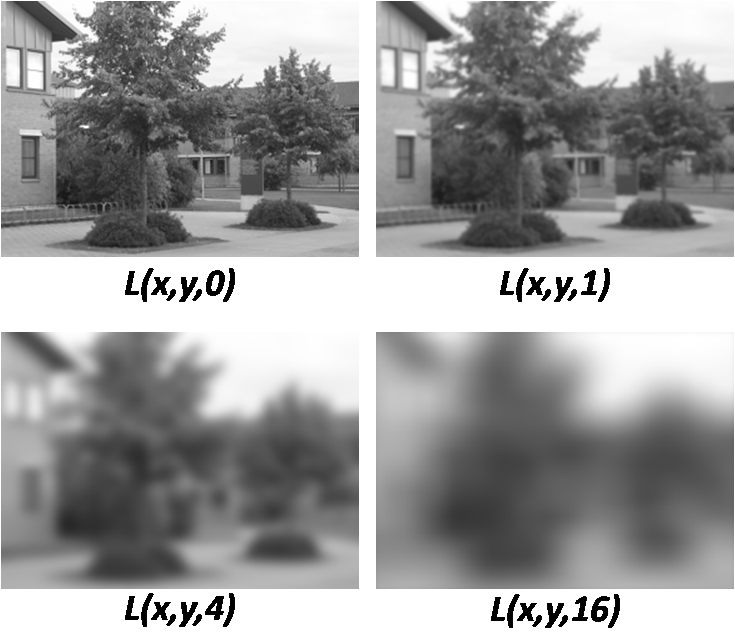
\includegraphics[width=10cm]{ScaleSpaceRepresentation}
	\centering
	\caption{Reprezentacja przestrzeni skali dla różnych wartości $\sigma$}
	\label{im: Scale Space Representation}
\end{figure} 

Problem sprowadza się do znalezienia takiego zbioru operatorów $\tau_s$, który operaując na obrazie oryginalnym zdefiniuje zbiór obrazów rozmytych:  

Gaussowska przestrzeń skali (dla obrazu dwuwymiarowego) zdefiniowana jest jako splot obrazu \textit{I(x,y)} z dwuwymiarową funkcją Gaussa \textit{g(x,y,$\sigma$)}:
\begin{equation}
L(x,y,\sigma) = g(x,y,\sigma)*I(x,y)
\end{equation}
gdzie:
\begin{equation}
g(x,y,\sigma) = \frac{1}{2\pi\sigma}e^{-(x^2+y^2)/2\sigma}
\end{equation}

%Podany wzór spełniony jest dla \textit{$\sigma$$\geq$0}
Dla $\sigma = 0$ filtr Gaussa staje się funkcją impulsową, zatem \textit{L(x,y,0) = f(x,y)}. Wraz ze zwiększaniem parametru $\sigma$ przestrzeń skali \textit{L} staje się coraz bardziej rozmyta, czyli coraz mniej szczegółów przestaje być widoczne. Na rysunku \ref{im: Scale Space Representation} przedstawiono przykład tworzenia przestrzennej reprezentacji skali.

\section{Windows Presentation Foundation (WPF)}
\label{sec: WPF}
Windows Presentation Foundation jest silnikiem graficznym dostarczanym przez firmę Microsoft. Jego premiera nastąpiła w 2006 roku, gdy stał się częścią platformy programistycznej .NET w wersji 3.0.  Jest wykorzystywany głównie do budowania aplikacji okienkowych nowej generacji dla systemu opracyjnego Windows. WPF zbudowany został całkowicie niezależnie do dotychczasowego silnika renderujacego GDI. Dostarcza model programistyczny umożliwiajacy budowanie aplikacji oraz pozwalający na bezwzględną separację logiki biznesowej od interfejsu użytkownika. 

\begin{figure}[h]
	%\centering
	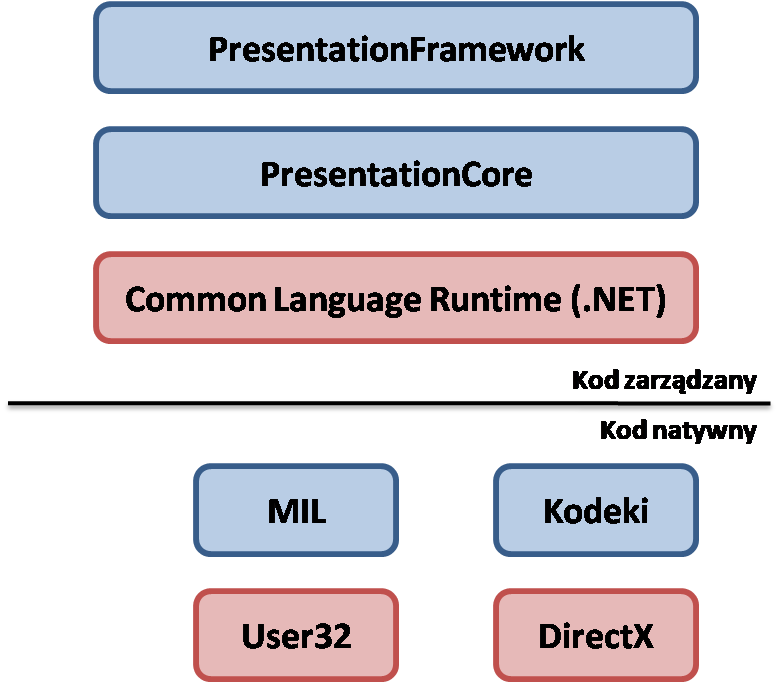
\includegraphics[width=10cm]{WpfArchitecture}
	\centering
	\caption{Architektura WPF. Czerwone elementy to komponenty bibliotek Windows. SKładowe WPF oznaczono kolorem niebieskim.}
	\label{im: WpfArchitecture}
\end{figure} 

Architektura silnika WPF została oparta zarówno o kod zarządzany, jak i o kod natywny.  Większość elementów składowych znajduje się w kodzie zarządzanym, tak jak publiczne API dostępne dla deweloperów. Na rysunku \ref{im: WpfArchitecture} przedstawiono architekturę silnika, w skład którego wchodzą:

\begin{itemize}
	\item PresentationFramework – biblioteka implementująca elementy do prezentacji dla końcowego uzytkownika tj. rozkład kontrolek, wyświetlanie animacji, skalowanie aplikacji. 
	
	\item PresentationCore – podstawowa biblioteka w technologii WPF. Dostarcza wraper dla MIL z poziomu kodu zarządzanego oraz impementuje bazowe  usługi dla każdej aplikacji WPF. W skład tych usług wchodzi przede wszystkim system zarządzania wiadomościami , którego implementację stanowi obiekt typu Dispacher.  
	
	\item Media Integration Layer, MIL – komponent działający w kodzie niezarządzanym w celu zapewnienia wydajnej współpracy  z DirectX.   Zawiera silnik kompozycji, który odpowiada za  podstawową obsługę renderowania powierzchni 2D oraz 3D.
	
	\item Kodeki – zbiór programów odpowiedzialnych do przekształcania strumienia danych do postaci multimedialnej.
	
	\item DirectX – kolekcja zawierająca interfejsy programistyczne aplikacji (z ang. application programming interfaces, APIs). Zestaw ten  wspomaga generację grafiki, dźwięku oraz innych elementów związanych z aplikacjami multimedialnymi
	
	\item User32 – komponent Microsoft Windows dostarczający bazowe funkcjonalności do tworzenia prostych interfejsów użytkownika.  Aplikacje WPF zawierają obiekt typu Dispacher, który używa systemu zarządzania wiadomościami dostępnymi w User32.
	
	\item Common Language Runtime, CLR – wspólne środowisko uruchomieniowe. Podstawowy komponent .NET. Pelni wiele kluczowych roli tj. uruchomienie aplikacji, zarządzanie pamięcią. Dodatkowo zajmuje się również konwersja języka IL do kodu maszynowego. Elementem bazowym środowiska CLR jest standardowy zestaw typów danych, który jest wykorzystywany przez wszyskie języki programowania oparte o CLR. 
	
\end{itemize}

Silnik WPF udostępnia system własności dla obiektów, które dziedziczą z DependencyObject. Obiekt ten monitoruje  wszytkie zależności pomiędzy własnościami i jest w stanie wykonywać odpowiednie akcje bazujac na ich zmianach. Własności implementują mechanizm informujący o zmianach (z ang. Change notifications), który wywołuje wbudowane zachowania (z ang. Behaviors) w przypadku wykrycia jakiejkolwiek zmiany. Dodatkowo isniej możliwość definiowania własnych zachowań w celu propagowania informacji o zmianie własności do innych elementów . System zarządzania rozkładem elementów w obrzarze interfejsu użytkownika wykorzystuje powyższy zbior zachowań do przeliczania nowego rozkładu w przypadku zmiany własności. Dzięki temu architektura systemu WPF spełnia deklaratywny paradygmat programowania, w którym praktycznie wszystko, począwszy od ustawania wielkości kontrolek do tworzenia animacji może zostać osiągnięte poprzez zmianę własności. Takie zachowanie umożliwia tworzenie aplikacji WPF w XAML (z ang. Extensible Application Markup Language) – deklaratywnym języku znaczników, gdzie przy pomocy atrybutów oraz słów kluczowych tworzone jest bezpośrednie połączenie z własnościami oraz klasami technologii WPF. 

Każdy element interfejsu aplikacji WPF dziedziczy z abstrakcyjnej klasy Visual. Obiekty tej klasy dostarczają interfejs do drzewa kompozycji zarządzanego przez MIL. Każdy element WPF tworzy oraz dodaje przynajmniej jeden węzeł kompozycji do drzewa. Węzły te zawierają przede wszystkim instrukcje renderowania takie jak przycinanie elementu bądź transformacja wizualna. Zatem cała aplikacja może być traktowana jako kolekcja węzłów kompozycji, które są przechowywane w buforze pamięci. Okresowo MIL przechodzi po strukturze drzewa i wykonuje instrukcje renderowania dla każdego węzła. Powoduje to tworzenie kompozytu na powierzchni DirectX, która następnie jest wyświetlana na ekranie.  MIL wykorzystuje algorytm malarza, w którym wyświetlanie elementów na monitorze rozpoczyna się od tych najbardziej odległych (tło). Takie zachowanie umożliwia renderowanie złożonych efektów takich jak rozmycie czy transparentność. Dodatkowo proces rysowania jest sprzętowo wspomagany przy pomocy GPU. 

Każda z aplikacji WPF staruje z dwoma wątkami: pierwszy służy do obsługi interfejsu użytkownika, a drugi, działający w tle, obsługuje renderowanie oraz przerysowywanie – jego działanie jest automatyczne, więc nie wymaga żadnej interwencji dewelopera. Wątek powiązany z UI przechowuje obiekt Dispacher’a (poprzez instancję klasy DispacherObject), który zajmuje się kolejkowaniem operacji koniecznych do wykonania na interfejsie użytkownika.

Etap tworzenia układu interfejsu użytkownika podzielony jest na dwie fazy: Mierzenie (z ang. Measure) oraz Porządkowanie (z ang. Arrange). Faza mierzenia rekursywnie wywołuje wszystkie elementy określa rozmiar, z jakim one będą wyświetlane. Porządkowanie to faza, podczas której następuje rekursywne układanie wszystkich elementów w stosunku do ich rodziców w drzewie kompozycji. 


\section{Algorytm SURF}
Algorytm SURF (skrót od ang. \textit{Speeded Up Robust Features}) został opatentowany przez grupę naukowców w 2007 roku [BIBLIOGRAFIA]. Należy do rodziny algorytmów bazujących na punktach kluczowych i służy do porównywania dwóch obrazów operując w odcieniach szarości. W celu znalezienia cech obrazu niezależnych od zmiany skali wykorzystuje opisaną w podrozdziale \ref{sec:StateSpace} technikę utworzenia ciągłej przestrzeni skali opartej na rozkładzie Gaussa. 
%Dodatkowo algorytm ten dzieli przestzeń skali na poziomy oraz oktawy. Oktawa odpowiada zbiorowi splotów, w którym wartość parametru $\sigma$ zostaje podwojona. Każda oktawa podzielona jest na jednakowo odległe (ze względu na parametr $\sigma$) poziomy. Przykład przedstawiono na rysunku \ref{im: OctavesAndLevels}.

Działanie algorytmu można podzielić na 3 etapy:
\begin{itemize}
	\item Detekcja (z ang. \textit{Detection}) – faza automatycznej identyfikcji punktów kluczowych (z ang. \textit{interest points}). Te same punkty powinny zostać wykryte niezależnie od zmian w położeniu, naświetleniu oraz orientacji obrazu, również w pewnym stopniu od zmiany skali oraz punktu widzenia. 
	\item Opis (z ang. \textit{Description}) – każdy punkt kluczowy powinien zostać opisany w unikatowy sposób., aby był niezależny od rotacji oraz przeskalowaniu obrazu.
	\item Zestawienie (z ang. \textit{Matching}) – faza, podczas której określa się (na podstawie podanych punktów kluczowych) jakie obiekty znajdują się na obrazie. 
\end{itemize}

W dalszej części rozdziału przedstawiono bardziej dokładną analizę dwóch pierwszych etapów.

\subsection{Detekcja}
Algorytm SURF do wykrycia punktów kluczowych wykorzystuje wyznacznik Hesjanu. Dokładniej rzecz ujmując, metoda ta wyszukuje na obrazie regionów, w których wyznacznik macierzy Hessego jest maksymalny. 






%Najważniejszy element detekcji to proces polegający na ograniczaniu lokalnych wartości niemaksymalnych (z ang. \textit{non-maximal suppression}) dla wyznaczników macierzy Hessego przy różnych wartościach parametru $\sigma$. W celu redukcji czasu obliczeń korzysta z obrazu całkowego opisanego w podrozdziale \ref{sec:IntegralImage}.

Mając do dyspozycji punkt \textit{\textbf{x}=(x,y)} z obrazu całkowego, macierz Hessego \textit{H(\textbf{x},$\sigma$)} dla skali $\sigma$ jest zdefiniowana następująco:
\begin{equation}\textsl{}
H(\textbf{x},\sigma) = 
\begin{bmatrix}
L_{xx}(\textbf{x},\sigma) & L_{xy}(\textbf{x},\sigma) \\ L_{xy}(\textbf{x},\sigma) & L_{yy}(\textbf{x},\sigma)
\end{bmatrix}
\end{equation}

gdzie 
\begin{equation}\textsl{}
L_{xx}(\textbf{x},\sigma) = I(\textbf{x})*\frac{\delta^2}{\delta x^2}g(\sigma)
\end{equation}
\begin{equation}\textsl{}
L_{xy}(\textbf{x},\sigma) = I(\textbf{x})*\frac{\delta^2}{\delta xy}g(\sigma)
\end{equation}

Udowodniono, że przestrzeń skali oparta o funkcję Gaussa jest rozwiązaniem optymalnym {BIBLIOGRAFIA}, jednakże w zastosowaniach praktycznych wyliczanie splotu jest niezwykle kosztowne obliczeniowo. W celu przyspieszenia obliczeń dokonano aproksymacji drugich pochodnych cząstkowych filtrami przedstawionymi na rysunku \ref{im: GaussianApproximation}. Dodatkowo wykorzystanie obrazu całkowego powoduje, że czas wyliczania splotów nie zależy od wielkości filtra. 
\begin{figure}[h]
	%\centering
	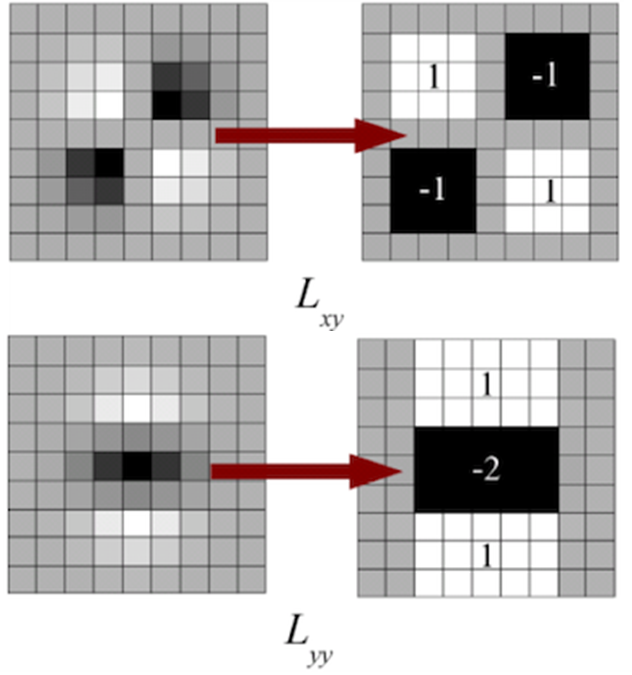
\includegraphics[width=8cm]{SurfLxyLyy}
	\centering
	\caption{Dwa rysunki po lewej to sploty \textit{$L_{xy}$} oraz \textit{$L_{yy}$} poddane dyskretyzacji oraz przycięciu. Po prawej stronie przedstawiono aproksymacje wyżej wymienionych splotów (odpowiednio \textit{$D_{xy}$} oraz \textit{$D_{yy}$}). Szare regiony są równe zero [BIBLIOGRAFIA]}
	\label{im: GaussianApproximation}
\end{figure}

Przedstawione filtry o rozmiarze \textit{9 x 9} odpowiadają splotom, dla których parametr $\sigma$ jest równy 1.2. Jest to najmniejsza wartość skali, dla której algorytm SURF może dawać zadowalające rezultaty.

Biorąc pod uwagę powyższe założenia, wyznacznik aproksymowanej macierzy Hessego wynosi:
\begin{equation}\textsl{}
det(H_{aproks}) = D_{xx}D_{yy} - (wD_{xy})^2.
\end{equation}
Aby uczynić aproksymację Hesjanu bardziej dokładną wprowadzono parametr \textit{w}. Teoretycznie jest on zależny od skali, jednakże badania wykazały [BIBLIOGRAFIA], że można uczynić go stałą równą \textit{0.9}.  
Wynikiem powyższych działań jest uzyskanie aproksymowanego wyznacznika Hesjanu dla każdego punktu obrazu \textit{\textbf{x}} przy różnych wartościach parametru $\sigma$.

 Algorytm SURF dzieli przestrzeń skali na oktawy. Oktawa reprezentuje zbiór odpowiedzi filtrów otrzymanych przez splot obrazu z filtrami coraz większych rozmiarów. Każda oktawa odpowiada fragmentowi przestrzeni skali, w którym nastąpiło podojenie parametru $\sigma$ oraz jest podzielona na stałą liczbę poziomów. Wraz ze wzrostem wielkości filtrów musi zostać spełnione dwa założenia: o istnieniu piksela centralnego oraz o zachowaniu proporcji poszczególnych obszarów maski. W pracy [BIBLIOGRAFIA] opisano szczegółowo, w jaki sposób definiować oktawy oraz liczbę poziomów dla nich. Przykład poprawnego skalowania filtra przedstawiono na rysunku \ref{im: FiltersScale}. 
 
 \begin{figure}[h]
 	%\centering
 	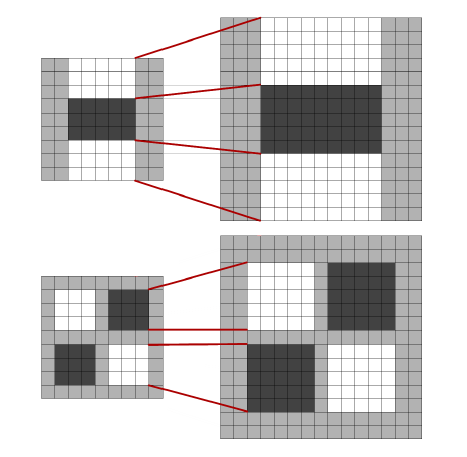
\includegraphics[width=12cm]{FiltersScale}
 	\centering
 	\caption{Filtr $D_{yy}$ oraz $D_{xy}$ dla dwóch kolejnych poziomów w oktawie (\textit{9 x 9} oraz \textit{15 x 15}). Długość czarnego regionu dla górnego filtra może zostać zwiększona tylko o parzystą liczbę pikseli w celu zagwarantowania istnienia piksela centralnego.}
 	\label{im: FiltersScale}
 \end{figure}
 
W celu zlokalizowania punktów kluczowych na obrazie we wszystkich skalach, algorytm SURF wykorzystuje ograniczanie lokalnych wartości niemaksymalnych (z ang. \textit{non-maximal suppression}) dla obszaru wielkości \textit{3 x 3 x 3} piksele. Zasada działania została opisana w pracy [BIBLIOGRAFIA]. Następnie maksima wyznacznika Hessjanu dla poszczególnych skal sa interpolowane na obraz oryginalny.

\subsection{Deskryptor} 
Aby punkt kluczowy był niewrażliwy na zmiany orientacji, punktowi przypisywana zostaje orientacja. W tym celu algorytm SURF wylicza odpowiedź falki Haara dla kolistego otoczenia punktu orientacji. Falka jest wyliczana w kierunku poziomym (\textit{dx}) oraz pionowym (\textit{dy}) dla każdego elementu z otoczenia punktu kluczowego.
Główna orientacja jest wyliczana następująco: mając odpowiedzi falki Haara dla każdego punktu z otoczenia, skonstruowano przesuwne okno o kącie rozwarcia równym 60 stopni. Dla każdego okna wyliczano sumę wszystkich elementów, a maska zostaje przesunięta. Najdłuższy znaleziony wektor stanowi główną orientację znalezionego punktu kluczowego. Szczegóły na rysunku \ref{im: SurfOrientationTwo}.

 \begin{figure}[h]
	%\centering
	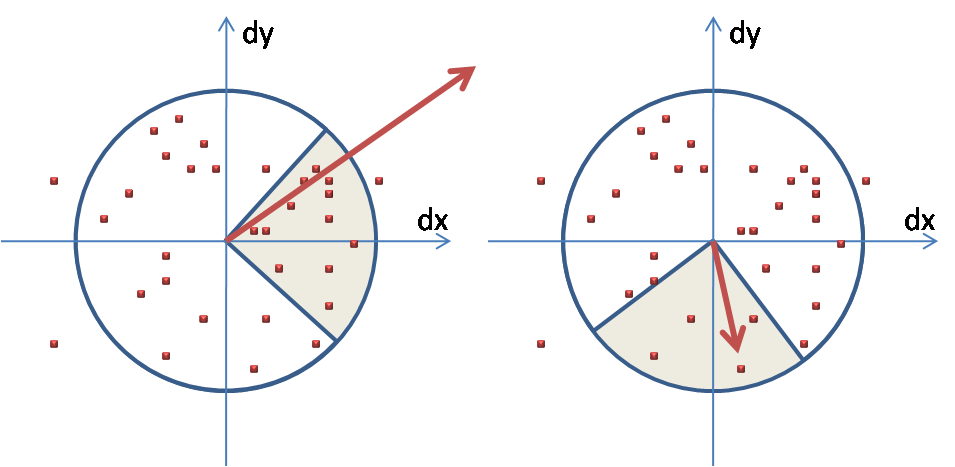
\includegraphics[width=12cm]{SurfOrientationTwo}
	\centering
	\caption{Przypisanie orientacji. Okno o kącie rozwarcia 60 stopni obraca się wokół początku układu współrzędnych, a wyliczone odpowiedzi falki Haara zostają sumowane tworząc wektory oznaczone kolorem czerwonym. Najdłuższy wektor determinuje główną orientację punku kluczowego.}
	\label{im: SurfOrientationTwo}
\end{figure}

Kolejnym etapem tworzenia deskryptora jest podzielenie obszaru wokół punktu kluczowego na  \textit{4 x 4} kwadratowe obszary. Taki podział zachowuje istotne przestrzenne informacje. Każdy z podregionów zawiera \textit{5 x 5} punktów rozmieszczonych regularnie w wierzchołkach siatki. Dla każdego punktu wyliczone zostają odpowiedzi falki Haara w kierunku poziomym oraz pionowym. Odpowiedzi te uwzględniają rotację całego obszaru zgodnie z orientacją badanego punktu kluczowego. Schemat przedstawiono na rysunku \ref{im: Description}. Następnie odpowiedzi \textit{dx} oraz \textit{dy} są sumowane dla każdego z podregionów. Stanowią one pierwszą część deskryptora cechy. Dodatkowo w celu uwzględnienia informacji o zmianach intensywności wyliczane są sumy modułów odpowiedzi falki Haara. 

Zatem, dla każdego z podregionów otrzymano czterowymiarowy wektor opisujacy o strukturze \textit{\textbf{v} = ($\sum$$d_x$, $\sum$$d_y$, $\sum$$|d_x|$, $\sum$$|d_y|)$}. Uwzględniając wszystkie podregiony, punkt kluczowy opisany jest 64-elementowym wektorem. 

 \begin{figure}[h]
	%\centering
	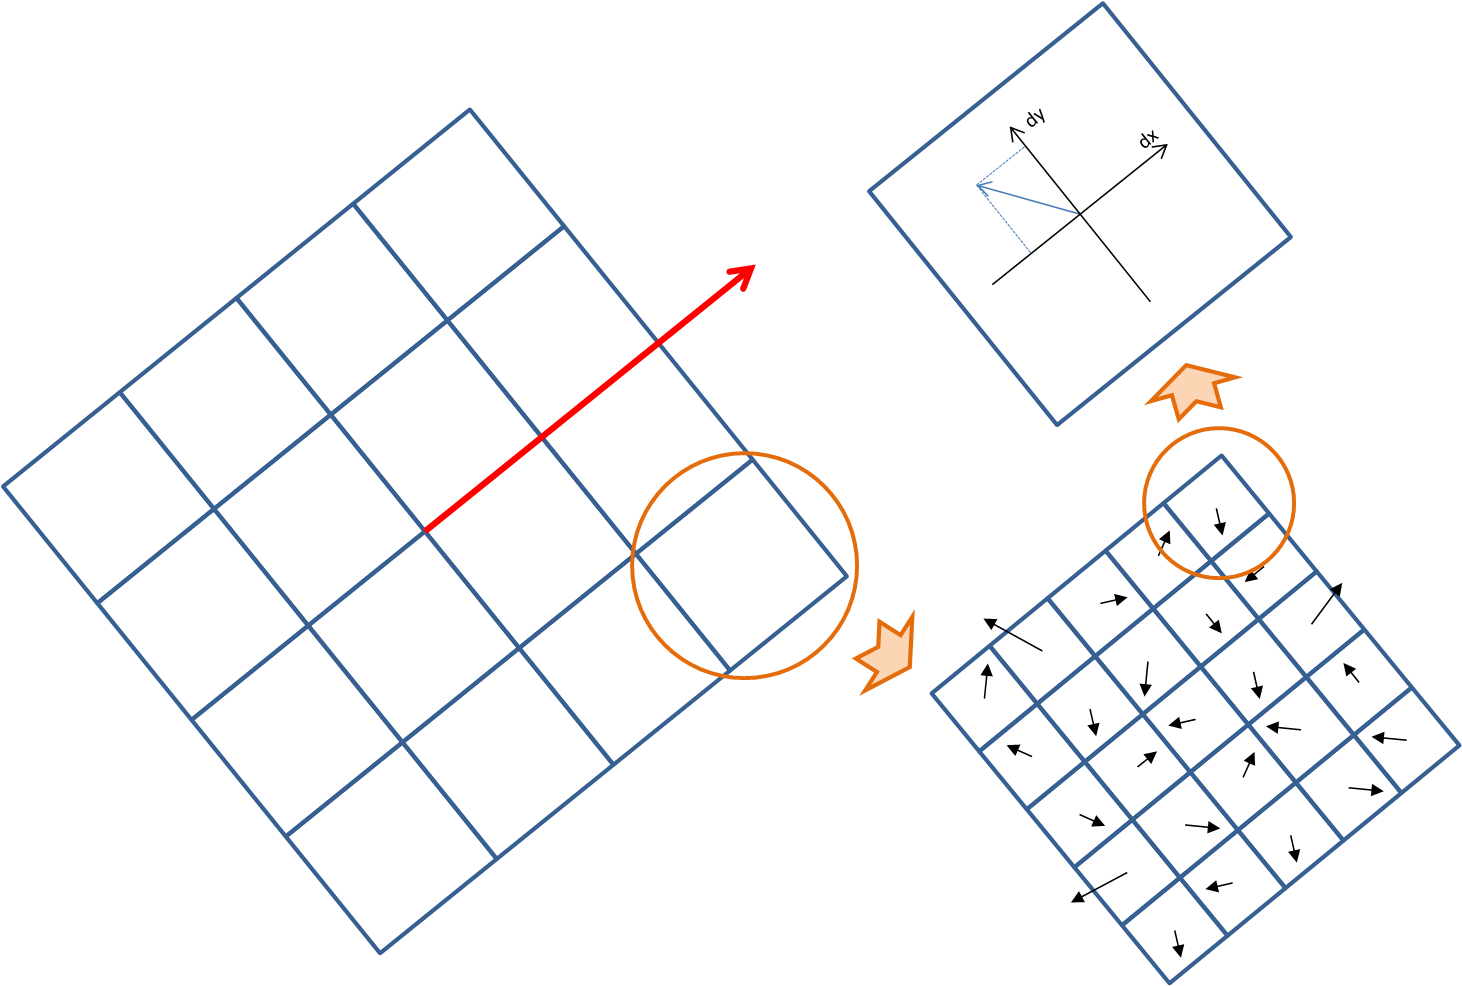
\includegraphics[width=16cm]{Description}
	\centering
	\caption{Tworzenie deskryptora. Otoczenie punktu kluczowego obrócono zgodnie z orientacją cechy. Dla wszystkich elementów podregionu wyliczono odpowiedź falki Haara w dwóch kierunkach.}
	\label{im: Description}
\end{figure}

MOŻNA DOPISAC O ZNAKU LAPLASJANU I O ROZRZERZENIU DO 128 ELEMENTOW.

\section{Accord .NET}
Accord .NET jest to szkielet aplikacyjny oparty o środowisko .NET. Zawiera biblioteki implementujące bardzo wiele algorytmów z szerokiej listy dziedzin nauki takich jak:

\begin{itemize}
	\item klasyfikacja: sieci neuronowe, metody wektorów nośnych (z ang. Support Vector Machine, SVM), algorytm Levenberga-Marquardta, model Markova, tworzenie drzew decyzyjnych
	\item regresja: regularyzacja, regresja liniowa, wielomianowa, 
	\item analiza skupień (z ang. \textit{clustering}): algorytm k-średnich, podział binarny. 
	\item rozkład prawdopodobieństwa: rozkład normalny, Poissona, Cauchy'ego
	\item Przetwarzanie obrazów cyfrowych (z ang. \textit{digital image processing, DIP}): deskryptory punktów kluczowych - SURF, FREAK, FAST; deskryptory gęstości - HOG, LBP
	\item Rozpoznawanie obrazów (z ang. computer vision): metody do detekcji, śledzenia oraz transformacji obiektów w strumieniu wideo. 
\end{itemize}

Szkielet ten został zaimplementowany aby rozszerzyć możliwości istniejącego rozwiązania - AForge .NET, jednak z czasem oba podmioty zostały ze sobą połączone pod jedną nazwą Accord .NET. Framework jest dostępny do pobrania z poziomu kodu zródłowego jak również za pomocą systemu zarządzania pakietami - \textit{NuGet}.

\section{C\#}
 C\# jest językiem programowania spełniającym wiele paradygmatów takich jak programowanie funkcyjne, obiektowe, imperatywne czy generyczne. Został utworzony przez firmę \textit{Microsoft} wewnątrz platformy .NET i zatwierdzony jako standard przez ISO (ISO/IEC 23270:2006) oraz Ecma (ECMA-334). Jest jednym z języków wchodzącym w skład Architektury Wspólnego Języka (z ang. \textit{Common Language Infrastructure, }). Najnowsza wersja języka to C\# 7.3, która ukazała się w 2018 roku wraz z środowiskiem programistycznym \textit{Visual Studio 2017} w wersji 15.7.2.
 Przykładowe cechy języka C\#:
 \begin{itemize}
 	\item C\# z założenia ma być językiem prostym, nowoczesnym, obiektowym
 	\item Język posiada hierarchię klas, a wszystkie elementy (nawet najprostsze typy) dziedziczą z klasy \textit{System.Object}.
 	\item Język ma zapewniać wsparcie w tworzeniu oprogramowania, w skład którego wchodzą: sprawdzanie silnego typowania, kontrola zakresu tablic, detekcja prób użycia niezainicjowanych zmiennych.
 	\item Automatyczne odśmiecanie pamięci (usuwanie nieużywanych elementów) - wykorzystanie mechanizmu \textit{Garbage Collector}.
 	\item Wielodziedziczenie, czyli dziedziczenie od więcej niż jednej klasy jest niedozwolone. Wielokrotne dziedziczenie jest możliwe jedynie po interfejsach.
 	\item Wsparcie dla internacjonalizacji.
 	\item Przenośność oprogramowania oraz łatwość wdrożenia w rozproszonych środowiskach. 
 	\item Język C\# jest bezpieczny w kontekście konwersji typów. Automatyczna konwersja jest dokonywana tylko w przypadku, gdy dane rzutowanie jest uznawane za bezpieczne.
 	\item Mechanizm refleksji oraz dynamicznego tworzenia kodu. Takie wsparcie umożliwia tworzenie oprogramowania, którego części nie jest w całości znane podczas kompilacji.
 	Takie działanie jest szeroko wykorzystywane w procesie mapowania obiektowo-relacyjnego (z ang. Object-Relational Mapping, ORM).
 \end{itemize} 

\section{.NET}
Platforma programistyczna .NET została zaprojektowana przez firmę \textit{Microsoft}. Zawiera w sobie obszerną bibliotekę klas FCL (z ang. \textit{Framework Class Library}) oraz zapewnia kompatybilność dla kilku języków programowania. Programy napisane z wykorzystaniem .NET są wykonywane w środowisku CLR (z ang. \textit{Common Language Runtime}) - jest to maszyna wirtualna, która dostarcza usługi takie jak bezpieczeństwo, zarządzanie pamięcią czy obsługę wyjątków. 
W skład architektury wchodzą: MOŻNA COS DOPISAĆ


Cechy platformy .NET:
\begin{itemize}
	\item Głównym elementem platformy .NET jest Środowisko Uruchomieniowe Wspólnego Języka (z ang. \textit{Common Language Runtime}, CLR). Stanowi ono implementację CLI gwarantując wiele właściwości oraz zachowań w obszarach zarządzania pamięcią bądź bezpieczeństwa. Głównym zadaniem komponentu CLR jest zamiana skompilowanego kodu CIL (z ang. Common Intermediate Language) na kod maszynowy, który jest dostosowany do maszyny, na jakiej został uruchomiony. MOŻE RYSUNEK?
	\item Kompatybilność wsteczna: ponieważ systemu komputerowe bardzo często wymagają interakcji pomiędzy nowszymi i starszymi komponentami, platforma .NET daje możliwość wykonywania funkcji poza platformą. Dostęp do komponentów COM jest możliwy dzięki wykorzystaniu przestrzeni nazw \textit{System.Runtime.InteropServices} oraz \textit{System.EnterpriseServices}.
	\item W skład platformy .NET wchodzi komponent CTS (z ang. \textit{Common Type System}), który definiuje wszystkie możliwe typy danych wspierane przez CLR oraz w jaki sposób mogą one ze sobą ingerować. Dzięki temu jest możliwa wymiana typów bądz instancji obiektów pomiędzy bibliotekami oraz aplikacjami napisanymi w różnych językach opartych o .NET.
	\item Przenośność: platforma została zaprojektowana w taki sposób, aby jej implementacja była możliwa dla różnych systemów operacyjnych.
	\item Bezpieczeństwo: platforma .NET dostarcza wspólny model bezpieczeństwa dla programów tworzonych w jej ramach. Została zaprojektowana w taki sposób, aby uniknąć wielu problemów z bezpieczeństwem aplikacji, do których należy m.in. przepełnienie bufora, które jest bardzo często używane przez złośliwe oprogramowanie (z ang. \textit{malicious software}, w skrócie \textit{malware}).
	
\end{itemize}

\section{Microsoft Visual Studio}
Microsoft Visual Studio to zintegrowane środowisko programistyczne (z ang. \textit{Integrated Deveopment Environment, IDE}) dostarczane prze firmę \textit{Microsoft}. Służy do budowania aplikacji konsolowych, jak również stron internetowych, aplikacji webowych oraz mobilnych. Visual Studio używa dostarczanych przez firmę Microsoft platform do tworzenia oprogramowania, do których należą m.in Windows Forms oraz Windows Presentation Foundation. Umożliwia tworzenie oprogramowania w 36 różnych językach programowania tj: C\#, C, C++, Visual Basic .NET, JavaScript czy CSS. Obecnie najnowsza wersja to Visual Studio 2017. 

Jednym z najważniejszych elementów wchodzących w skład środowiska jest edytor kodu. Jak każde IDE, Visual Studio zawiera edytor umożliwiający podświetlanie składni oraz auto-uzupełnianie brakujących fraz wykorzystując mechanizm \textit{IntelliSense}. Środowisko programistyczne wspiera tzw. kompilację w tle. W trakcie pisania kodu, Visual Studio kompiluje kod w tle w celu dostarczenia informacji o składni oraz ewentualnych błędach kompilacji. 

Visual Studio zawiera debugger umożliwiający redukcję błędów w oprogramowaniu zarówno dla kodu zarządzanego, jak i natywnego. Dodatkowo istnieje możliwość dopięcia debuggera do procesu w celu monitorowania zachowania. Visual Studio umożliwia dokonywania zrzutów pamięci (z ang. \textit{memory dumps}) jak również wczytywania ich w dalszych momentach debugowania. Debugger umożliwia tworzenie punktu wstrzymania (z ang. \textit{breakpiont}) - miejsca celowego zatrzymania wykonywania programu w celu analizy jego zachowania. Dodatkowo punkty wstrzymania mogą być warunkowe, czyli zatrzymanie w punkcie następuje w momencie spełnienia warunku. Debugger wspiera tzw. "Edytuj i Kontynuuj" - jak nazwa sugeruje, istnieje możliwość zmiany wartosci zmiennej podczas procesu debugowania.

Visual Studio zawiera narzędzia do tworzenia interfejsu użytkownika. Jeden z przykładów może stanowić narzędzie \textit{Cider} pomocne w budowaniu aplikacji WPF. Umożliwia tworzenie aplikacji poprzez przeciąganie istniejących elementów z przybornika oraz ustawianiu ich własciwości w dedykowanym oknie. Ponadto istnieje możliwość edycji widoku z poziomu języka znaczników XAML. Szczegółowy opis technologii WPF znajduje się w podrozdziale \ref{sec: WPF}.\textsl{}

\section{Algorytm centroidów}
Algorytm K-średnich (z ang. \textit{K-means}) jest jedną z najprostszych metod klasyfikacji bez nadzoru (z ang. \textit{unsupervised learning}). Grupowanie elementów oparte jest o wstępne podzielenie zbioru danych na z góry założoną liczbę klastrów. W kolejnych krokach niektóre z elementów skupień są przenoszone do innych klastrów w taki sposób, aby wariancja wewnątrz każdej z grup była jak najmniejsza. Minimalizacja wartosci wariancji powoduje, że elementy wewnątrz poszczególnych klastrów są do siebie maksymalnie podobne. 

\begin{enumerate}
	\item Wybór centroidów klastrów: dla podanej z góry liczby klas (skupień)  środki klastrów powinny zostać dobrane w taki sposób, aby były możliwie jak najdalej od siebie.
	\item Przyporządkowanie każdego elementu ze zbioru danych do najbliższego środka klastra, normę może stanowić odległość euklidesowa lub Czebyszewa.
	\item Ponowne wyliczenie środków skupień: w większości zastosowań nowym środkiem klastra jest punkt o współrzędnych stanowiących średnią arytmetyczną elementów wewnątrz skupienia.
	\item Powtarzanie algorytmu do momentu osiągnięcia kryterium zbieżności: sytuacja, podczas której środki klastrów pozostają bez zmian bądź nie zmienia się przynależność elementów do klas.
\end{enumerate}

Na rysunku \ref{im: Clustering} przedstawiono graf przepływu wyjaśniający zasadę działania algorytmu K-średnich.
\begin{figure}[h]
	%\centering
	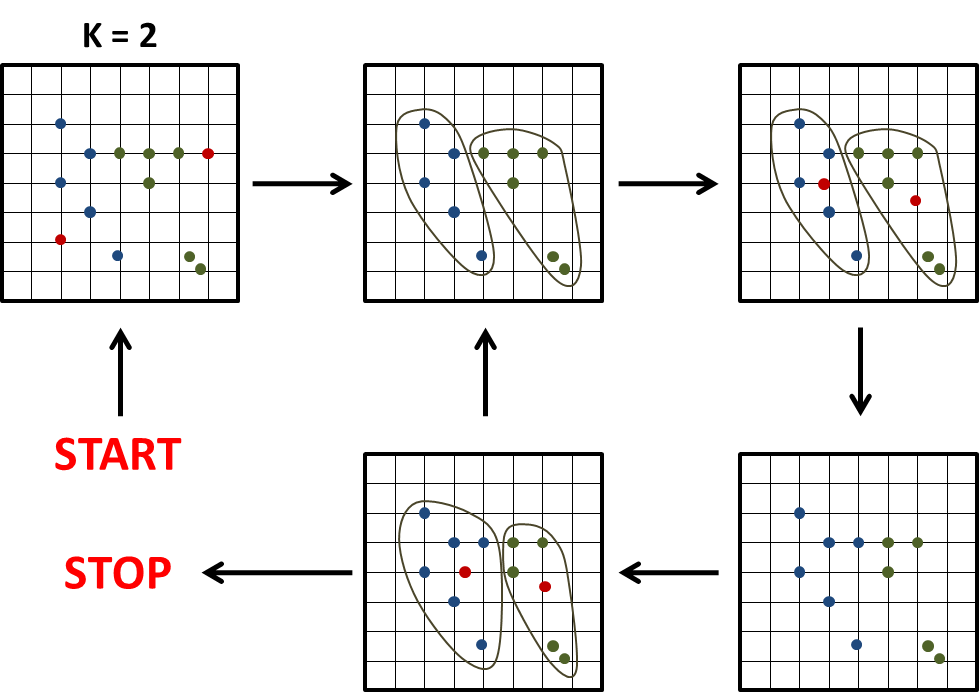
\includegraphics[width=16cm]{Clustering1}
	\centering
	\caption{Algorytm K-średnich. Pierwszy etap to wybór środków dla klastrów. Następnie dokonywane jest przypisanie punktów do odpowiedniej klasy. Kolejny etap to ponowne wyliczenie centroidów oraz reorganizacja klastrów. Algorytm działa dopóki środki klas ulegają zmianie.}
	\label{im: Clustering}
\end{figure}


\section{Metoda Wektorów Nośnych}
Metoda wektorów nośnych (z ang. \textit{Support Vector Machine}, SVM) to jeden z modeli uczenia maszynowego służący do klasyfikacji danych. Model SVM po raz pierwszy został opublikowany przez dwóch naukowców: Vladimira N. Vapnika oraz Alexey'a Chervonenkisa w 1963 roku. Może zostać użyty do rozwiązywania takich problemów jak rozpoznawanie tekstu pisanego czy klasyfikacja obrazów.

Mając do dyspozycji zbiór punktów uczących, w którym każdy z elementów należy do jednej z dwóch klas, SVM tworzy model, który przypisuje próbki testowe do jednej z dwóch kategorii. Model SVM jest reprezentowany jako zbiór punktów na przestrzeni skonstruowany w taki sposób, aby istniała wyraźna przerwa oddzielająca elementy rożnych klas. W zależności od tego, po której stronie przerwy próbka testowa została umiejscowiona, do tej kategorii zostanie przypisana. Bardziej formalnie SVM konstruuje hiperpłaszczyznę rozdzielającą zbiór próbek uczących. Najlepsza separacja zachodzi wtedy, gdy odległość hiperpłaszczyzny od najbliższego elementu dla każdej z klas jest maksymalna. 

Zbiór $n$-punktów uczących opisano następująco:
\begin{equation}
(\vec{x}_1,y_1), ..., (\vec{x}_n,y_n)
\end{equation}
gdzie $\vec{x}_i$ oznacza \textit{\textbf{p}}-wymiarowy wektor. Zmienna $y_i$ przyjmuje wartości -1 bądź 1 w zależności od tego, do której kategorii należy $\vec{x}_i$. Równianie płaszczyzny może zostać opisane następująco:
\begin{equation}
\vec{w}\cdot \vec{x} - b = 0
\end{equation}
gdzie $\vec{w}$ oznacza wektor normalny do szukanej hiperpłaszczyzny. W przypadku, gdy zbiór danych może być separowany liniowo, istnieje możliwość wyboru dwóch równoległych hiperpłaszczyzn, których odległość względem siebie jest maksymalna. Region leżący pomiędzy tymi hiperpłaszczyznami jest nazywany \textit{marginesem}, a optymalna hiperpłaszczyzna leży w jego połowie. Równania dla dwóch równoległych hiperpłaszczyzn są opisane następująco:
\begin{equation}
\vec{w}\cdot \vec{x}_i - b = 1
\end{equation}
\begin{equation}
\vec{w}\cdot \vec{x}_i - b = -1
\end{equation}
Dystans pomiędzy dwoma hiperpłaszczyznami jest równy $2 /||\vec{w}||$. Zatem w celu maksymalizacji dystansu pomiędzy płaszczyznami należy dokonać minimalizacji $||\vec{w}||$. Dodatkowo wymuszono obecność dowolnej próbki po właściwej stronie marginesu używając następujących zależności:
\begin{equation}
\vec{w}\cdot \vec{x}_i - b \geq 1 \hspace{0.5cm} dla \hspace{0.5cm} y_i = 1 
\end{equation}
\begin{equation}
\vec{w}\cdot \vec{x}_i - b \leq -1 \hspace{0.5cm} dla \hspace{0.5cm} y_i = -1
\end{equation}
Powyższe nierówności mogą zostać przekształcone do:
\begin{equation}
y_i(\vec{w}\cdot \vec{x}_i - b) \geq 1 \hspace{0.5cm} dla \hspace{0.2cm} wszystkich \hspace{0.2cm} 1 \leq i \leq n
\end{equation}
Zadanie minimalizacji może zostać postawione w następujący sposób:
"Minimalizacja normy wektora $\vec{w}$ dla zależności $y_i(\vec{w}\cdot \vec{x}_i - b) \geq 1$ dla $i=1 \ldots n$".
Szczegóły tworzenia hiperprzestrzeni w dwóch wymiarach przedstawiono na rysunku \ref{im: SvmMargin}
\begin{figure}[h]
	%\centering
	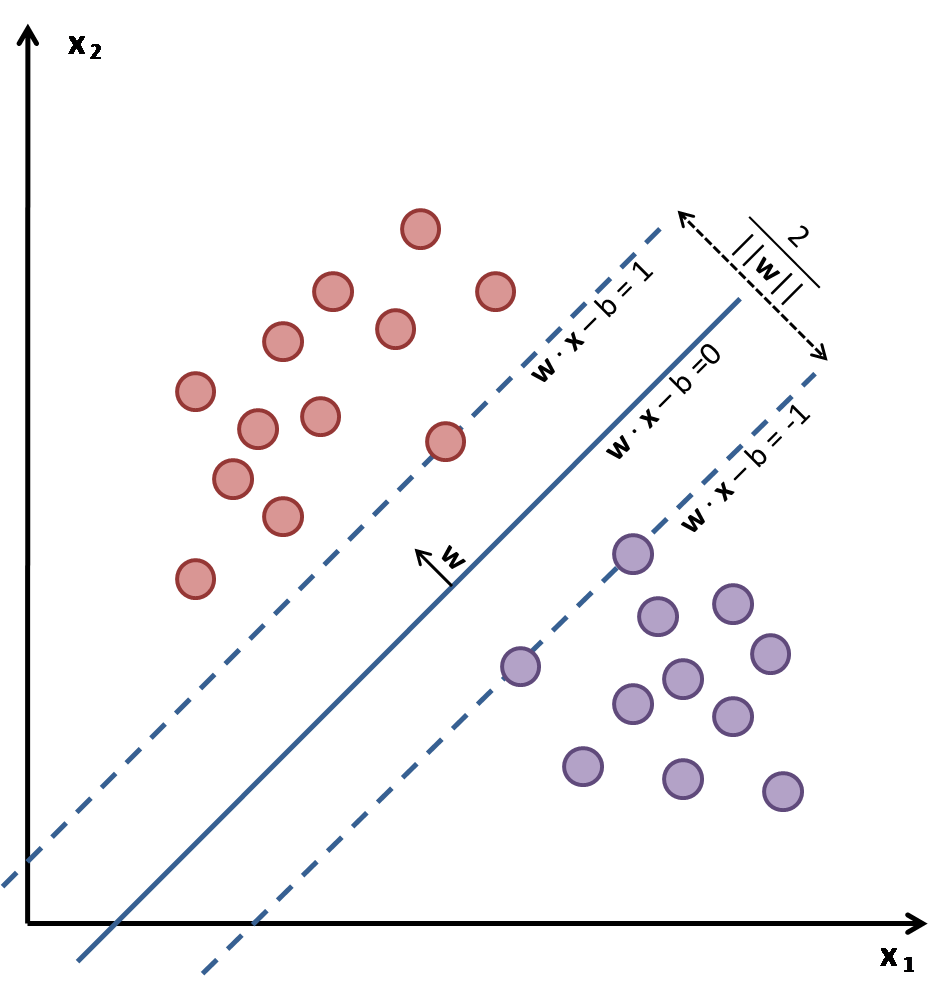
\includegraphics[width=12cm]{SvmMargin}
	\centering
	\caption{Sposób wyznaczania optymalnej hiperpłaszczyzny.}
	\label{im: SvmMargin}
\end{figure}

Oryginalny algorytm do szukania hiperpłaszczyzny rozdzielającej z maksymalnym marginesem stworzony w 1963 roku był liniowym klasyfikatorem. Jednakże w latach 90-tych Vapnik przy wsparciu innych naukowców zaproponował sposób umożliwiający konstrukcję nieliniowego klasyfikatora przez zastosowanie tzw. \textit{"kernel trick"}. Algorytm w swoim działaniu jest bardzo podobny do oryginału z tą różnicą, że każdy iloczyn skalarny zostaje zastąpiony przez nieliniową funkcję jądra. Do najbardziej znanych funkcji jądra należą:

\begin{itemize}
	\item Wielomianowa jednorodna: 
	\begin{equation}
	k(\vec{x}_i,\vec{x}_j) = (\vec{x}_i \cdot \vec{x}_j)^d
	\end{equation}
	\item Wielomianowa niejednorodna:
	\begin{equation}
	k(\vec{x}_i,\vec{x}_j) = (\vec{x}_i \cdot \vec{x}_j + 1)^d
	\end{equation}
	\item Jądro RBF (z ang. Radial Basis Funcion):
	\begin{equation}
	k(\vec{x}_i,\vec{x}_j) = \exp\bigg( -\frac{||\vec{x}_i - \vec{x}_j||^2}{2\sigma^2}\bigg)
	\end{equation}
\end{itemize}
Przykład zastosowania funkcji jądra przedstawiono na rysunku \ref{im: KernelMachine}.
\begin{figure}[h]
	%\centering
	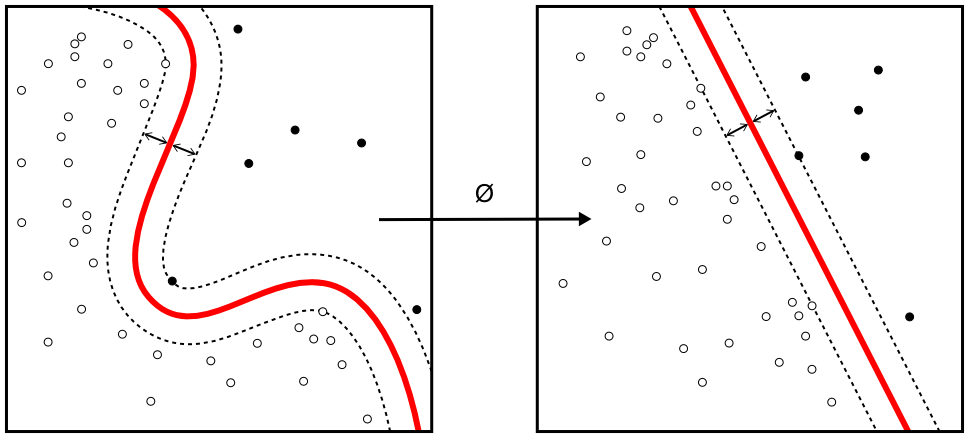
\includegraphics[width=12cm]{KernelMachine}
	\centering
	\caption{Sposób wyznaczania optymalnej hiperpłaszczyzny.}
	\label{im: KernelMachine}
\end{figure}

Istnieje również sposób na klasyfikację elementów dla większej niż dwa liczby kategorii. 

Redukcja klasyfikacji dla wielu kategorii do problemu binarnego dla wielu przypadków. Isnieje
Jednym ze sposobów sprowadza się do redukcji problemu 
















